\documentclass{article}[18pt]
\ProvidesPackage{format}
%Page setup
\usepackage[utf8]{inputenc}
\usepackage[margin=0.7in]{geometry}
\usepackage{parselines} 
\usepackage[english]{babel}
\usepackage{fancyhdr}
\usepackage{titlesec}
\hyphenpenalty=10000

\pagestyle{fancy}
\fancyhf{}
\rhead{Sam Robbins}
\rfoot{Page \thepage}

%Characters
\usepackage{amsmath}
\usepackage{amssymb}
\usepackage{gensymb}
\newcommand{\R}{\mathbb{R}}

%Diagrams
\usepackage{pgfplots}
\usepackage{graphicx}
\usepackage{tabularx}
\usepackage{relsize}
\pgfplotsset{width=10cm,compat=1.9}
\usepackage{float}

%Length Setting
\titlespacing\section{0pt}{14pt plus 4pt minus 2pt}{0pt plus 2pt minus 2pt}
\newlength\tindent
\setlength{\tindent}{\parindent}
\setlength{\parindent}{0pt}
\renewcommand{\indent}{\hspace*{\tindent}}

%Programming Font
\usepackage{courier}
\usepackage{listings}
\usepackage{pxfonts}

%Lists
\usepackage{enumerate}
\usepackage{enumitem}

% Networks Macro
\usepackage{tikz}


% Commands for files converted using pandoc
\providecommand{\tightlist}{%
	\setlength{\itemsep}{0pt}\setlength{\parskip}{0pt}}
\usepackage{hyperref}

% Get nice commands for floor and ceil
\usepackage{mathtools}
\DeclarePairedDelimiter{\ceil}{\lceil}{\rceil}
\DeclarePairedDelimiter{\floor}{\lfloor}{\rfloor}

% Allow itemize to go up to 20 levels deep (just change the number if you need more you madman)
\usepackage{enumitem}
\setlistdepth{20}
\renewlist{itemize}{itemize}{20}

% initially, use dots for all levels
\setlist[itemize]{label=$\cdot$}

% customize the first 3 levels
\setlist[itemize,1]{label=\textbullet}
\setlist[itemize,2]{label=--}
\setlist[itemize,3]{label=*}

% Definition and Important Stuff
% Important stuff
\usepackage[framemethod=TikZ]{mdframed}

\newcounter{theo}[section]\setcounter{theo}{0}
\renewcommand{\thetheo}{\arabic{section}.\arabic{theo}}
\newenvironment{important}[1][]{%
	\refstepcounter{theo}%
	\ifstrempty{#1}%
	{\mdfsetup{%
			frametitle={%
				\tikz[baseline=(current bounding box.east),outer sep=0pt]
				\node[anchor=east,rectangle,fill=red!50]
				{\strut Important};}}
	}%
	{\mdfsetup{%
			frametitle={%
				\tikz[baseline=(current bounding box.east),outer sep=0pt]
				\node[anchor=east,rectangle,fill=red!50]
				{\strut Important:~#1};}}%
	}%
	\mdfsetup{innertopmargin=10pt,linecolor=red!50,%
		linewidth=2pt,topline=true,%
		frametitleaboveskip=\dimexpr-\ht\strutbox\relax
	}
	\begin{mdframed}[]\relax%
		\centering
		}{\end{mdframed}}



\newcounter{lem}[section]\setcounter{lem}{0}
\renewcommand{\thelem}{\arabic{section}.\arabic{lem}}
\newenvironment{defin}[1][]{%
	\refstepcounter{lem}%
	\ifstrempty{#1}%
	{\mdfsetup{%
			frametitle={%
				\tikz[baseline=(current bounding box.east),outer sep=0pt]
				\node[anchor=east,rectangle,fill=blue!20]
				{\strut Definition};}}
	}%
	{\mdfsetup{%
			frametitle={%
				\tikz[baseline=(current bounding box.east),outer sep=0pt]
				\node[anchor=east,rectangle,fill=blue!20]
				{\strut Definition:~#1};}}%
	}%
	\mdfsetup{innertopmargin=10pt,linecolor=blue!20,%
		linewidth=2pt,topline=true,%
		frametitleaboveskip=\dimexpr-\ht\strutbox\relax
	}
	\begin{mdframed}[]\relax%
		\centering
		}{\end{mdframed}}
\lhead{Networks and Systems - Networks}


\begin{document}
\begin{center}
\underline{\huge Transport Layer II}
\end{center}
\section{Reliable data transfer}
We will:
\begin{itemize}
	\item Incrementally develop sender, receiver sides of reliable data transfer protocol (rdt)
	\item Consider only unidirectional data transfer - but control info will flow on both directions
	\item Use finite state machines (FSM) to specify sender, receiver
\end{itemize}
\begin{center}
	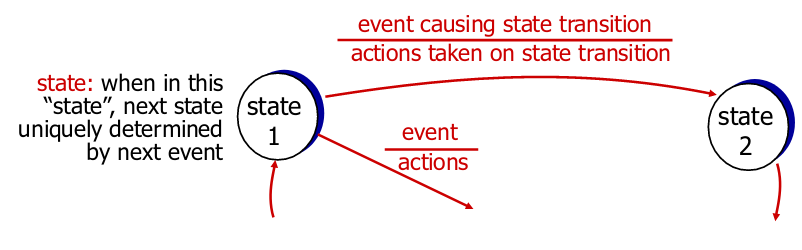
\includegraphics[scale=0.7]{rdt}
\end{center}
\subsection{rdt1.0: reliable transfer over a reliable channel}
Underlying channel perfectly reliable:
\begin{itemize}
	\item No bit errors
	\item No loss of packets
\end{itemize}
Separate FSMs for sender, receiver:
\begin{itemize}
	\item Sender sends data into underlying channel
	\item Receiver reads data from underlying channel
\end{itemize}
\begin{center}
	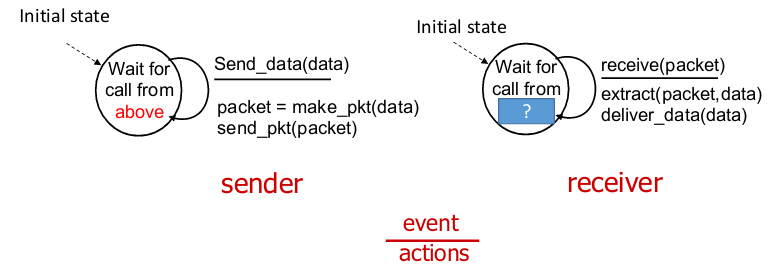
\includegraphics[scale=0.7]{rdt1}
\end{center}
\begin{important}[What layer is this in?]
This is happening in the transport layer
\end{important}
\subsection{rdt2.0}
\subsubsection{Channel with bit errors}
\begin{itemize}
	\item Underlying channel may flip bits in packet, checksum to detect bit errors
	\item The question: how to recover from errors:
	\begin{itemize}
		\item Acknowledgements (ACKs): receiver explicitly tells sender that packet received OK
		\item Negative acknowledgements (NAKs): receiver explicitly tells sender that packet had errors
		\item Sender retransmits packet on receipt of NAK
		\item Using ACKs and NAKs is known as ARQ (Automatic Repeat reQuest) protocols
		\begin{itemize}
			\item Error detection. Sender embeds extra bits in packets
			\item Feedback. Receiver provide sender with feedback
			\item Retransmission. Retransmit erroneous packets
		\end{itemize}
	\end{itemize}
	\item New mechanisms in \texttt{rdt2.0} (beyond \texttt{rdt1.0})
	\begin{itemize}
		\item Error detection
		\item Feedback: control msgs (ACK (1), NAK(0)) from receiver to sender
	\end{itemize}
\end{itemize}
\subsubsection{FSM specification}
\begin{center}
	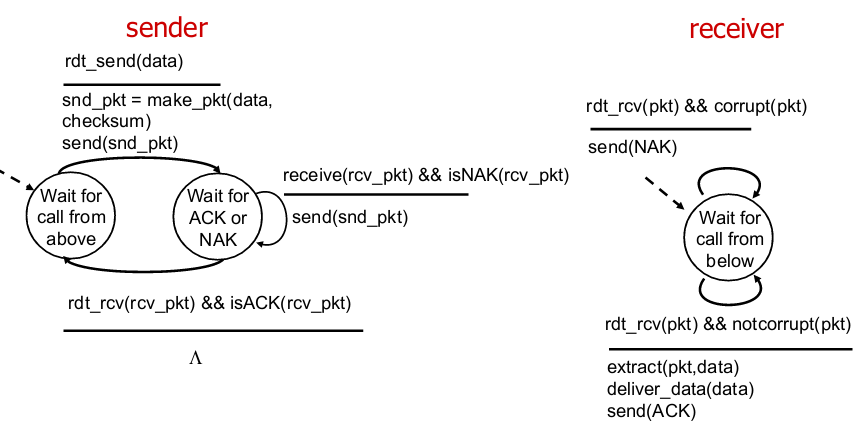
\includegraphics[scale=0.7]{FSM}
\end{center}
\subsubsection{Operation with no errors}
\begin{center}
	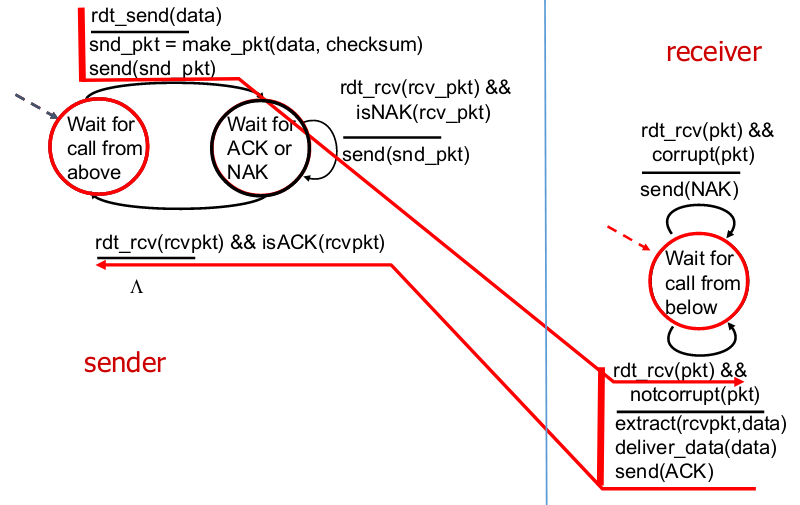
\includegraphics[scale=0.7]{operation_with_no_errors}
\end{center}
\subsubsection{Error scenario}
\begin{center}
	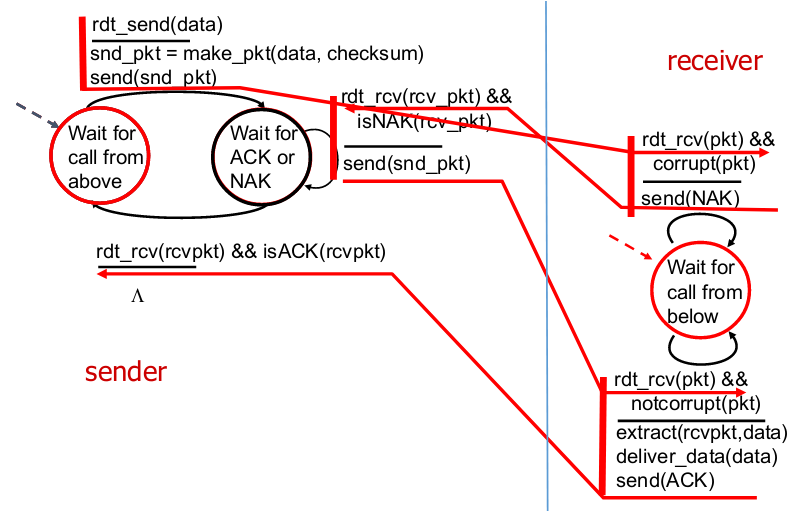
\includegraphics[scale=0.7]{error_scenario}
\end{center}
\subsubsection{Fatal flaw}
What happens if ACK/NAK corrupted:
\begin{itemize}
	\item Sender doesn't know what happened at receiver
	\item Can't just retransmit: possible duplicate
\end{itemize}
Handling duplicates:
\begin{itemize}
	\item Sender retransmits current packet if ACK/NAK corrupted
	\item Sender adds \textbf{sequence number} to each packet
	\item Receiver discards (doesn't deliver up) duplicate packet
\end{itemize}
Stop and wait:
\begin{itemize}
	\item Sender sends one packet, then waits for the receiver response
\end{itemize}
\subsection{rdt3.0}
\subsubsection{Channels with errors and loss}
New assumption:
\begin{itemize}
	\item Underlying channel can also lose packets (data, ACKs)
	\begin{itemize}
		\item Checksum, seq. \#, ACKs, retransmissions will be of help, but not enough
	\end{itemize}
\end{itemize}
Approach:
\begin{itemize}
	\item Sender waits "reasonable" amount of time for ACK
	\begin{itemize}
		\item Retransmits if no ACK received in this time
		\item If no packet (or ACK) just delayed (not lost):
		\begin{itemize}
			\item Retransmission will be duplicate, but seq. \#'s already handles this
			\item Receiver must specify seq \# of packet being ACKed
		\end{itemize}
		\item Requires countdown timer
	\end{itemize}
\end{itemize}
\subsubsection{Sender}
\begin{center}
	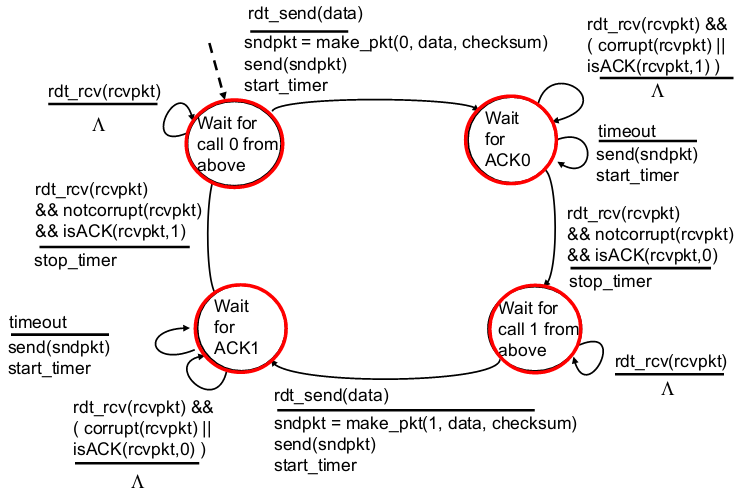
\includegraphics[scale=0.7]{rdt_sender}
\end{center}
\subsubsection{In action}
\begin{center}
	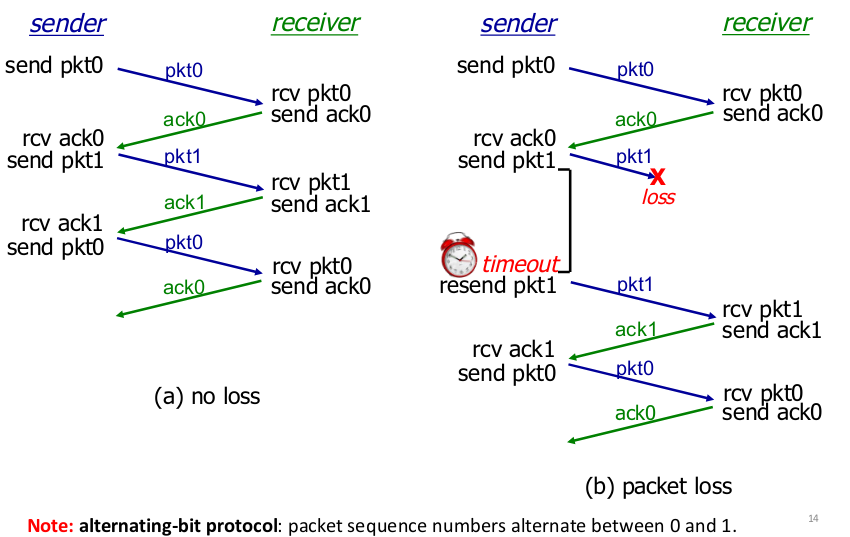
\includegraphics[scale=0.7]{rdt_in_action}
\end{center}
\begin{center}
	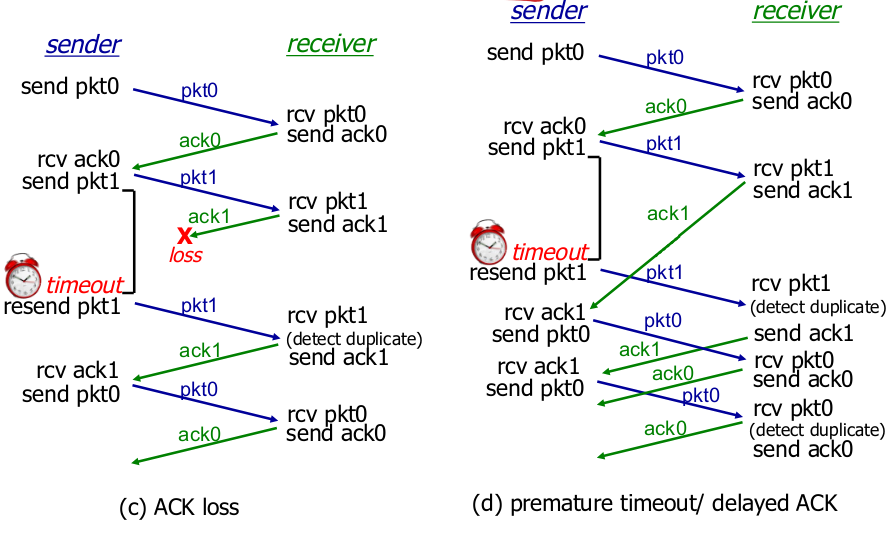
\includegraphics[scale=0.7]{rdt_in_action1}
\end{center}
\section{Pipelined protocols}
\begin{center}
	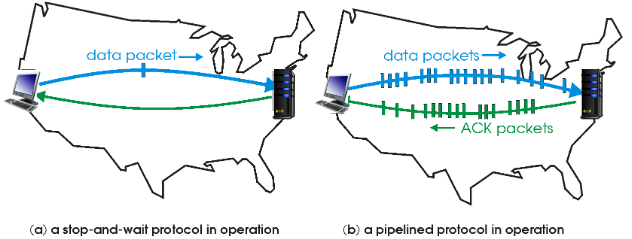
\includegraphics[scale=0.7]{pipelined_protocols1}
\end{center}
\textbf{Pipelining} has the following consequences for reliable data transfer protocols:
\begin{itemize}
	\item Range of sequence numbers must be increased
	\begin{itemize}
		\item Unique sequence number and there may be multiple, in-transit, unacknowledged packets
	\end{itemize}
	\item Multiple packet buffering at sender and/or receiver
	\begin{itemize}
		\item Sender buffers packets that have been transmitted but not yet acknowledged
		\item Buffering of correctly received packets
	\end{itemize}
	\item Range of sequence numbers needed and the buffering requirements will depend on the manner in which a data transfer protocol responds to lost, corrupted, and overly delayed packets
\end{itemize}
Two generic forms of pipelined protocols:

	\begin{defin} [Go-back-N]
	\begin{itemize}
		\item Sender can send multiple packets without waiting for ACK
		\item Sender can have up to N unacked packets in pipeline
		\item Receiver only sends cumulative ack, doesn't ack packet if there's a gap (so if it acks packet 4, it means it has packet 1,2,3 and 4)
		\item Sender has timer for oldest unacked packet, when timer expired, retransmit all unacked packets
	\end{itemize}
	\end{defin}
\begin{defin}[Selective repeat]
	\begin{itemize}
		\item Sender can have up to N unacked packets in pipeline
		\item Receiver sends individual ack for each packet
		\item Sender maintains timer for each unacked packet, when timer expires, retransmit only that unacked packet
\end{itemize}
\end{defin}

\subsection{GBN(Go Back N) in action}
\begin{center}
	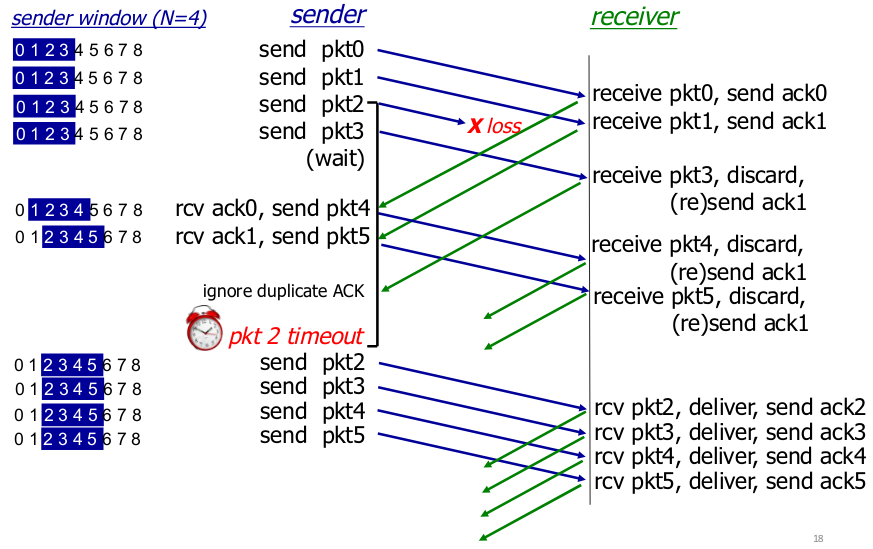
\includegraphics[scale=0.7]{GBN}
\end{center}
\subsection{Selective repeat}
\begin{itemize}
	\item Receiver individually acknowledges all correctly receives packets. Buffers packets, as needed, for eventual in-order delivery to upper layer
	\item Sender only resends packets for which ACK not received. Sender timer for each unACKed packet
	\item Sender window
	\begin{itemize}
		\item N consecutive seq \#'s
		\item Limits seq \#s of sent, unACKed packets
	\end{itemize}
\end{itemize}
\begin{minipage}{0.5\textwidth}
Sender:
\begin{itemize}
	\item Data from above:
	\begin{itemize}
		\item If next available seq \# in window, send packet
	\end{itemize}
	\item timeout(n)
	\begin{itemize}
		\item Resend packet n, restart timer
	\end{itemize}
	\item Mark packet n as received
	\item If n smallest unACKed packet, advance window base to next unACKed seq \#
\end{itemize}
\end{minipage}
\begin{minipage}{0.5\textwidth}
Receiver:
\begin{itemize}
	\item \texttt{packet n in [rcvbase, rcvbase+N-1]}
	\begin{itemize}
	\item Send ACK(n)
	\item Out-of-order: buffer
	\item In-order: deliver( also deliver buffered, in-order packets), advance window to next not-yet-received packet
	\end{itemize}
	\item \texttt{packet n in [rcvbase-N, rcvbase-1]}
	\begin{itemize}
		\item Ack(n)
	\end{itemize}
	\item Otherwise:
	\begin{itemize}
		\item Ignore
	\end{itemize} 
\end{itemize}
\end{minipage}
\subsubsection{Selective repeat in action}
\begin{center}
	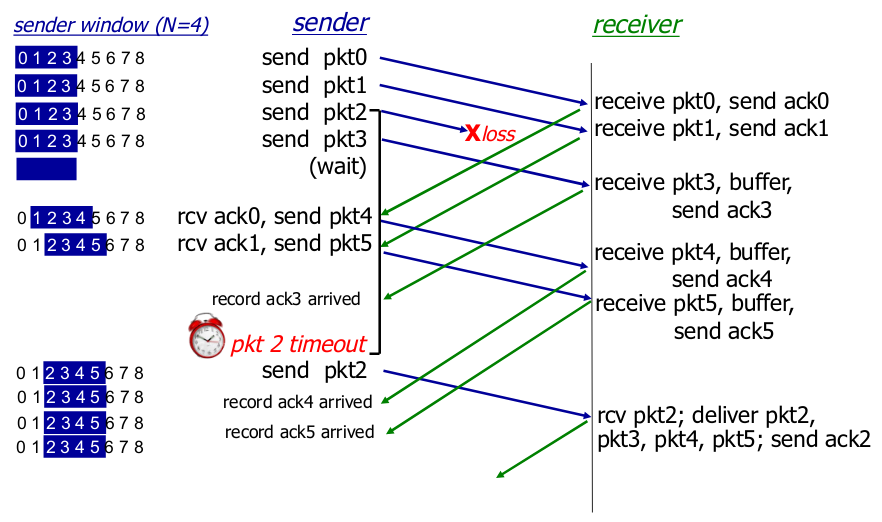
\includegraphics[scale=0.6]{selective_repeat_action}
\end{center}
\subsubsection{Selective repeat dilemma}
Example:
\begin{itemize}
	\item Finite range of seq \# s: 0,1,2,3
	\item Window size=3
	\begin{itemize}
		\item Receiver sees no difference in two scenarios
		\item Duplicate data accepted as new in (b)
	\end{itemize}
\end{itemize}
\begin{center}
	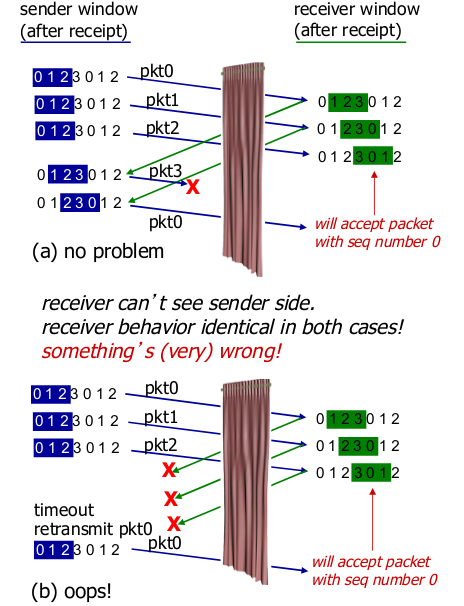
\includegraphics[scale=0.6]{selective_repeat_dilemma}
\end{center}
Note: That curtain is there to show that there is a lack of knowledge between the sender and receiver 

\end{document}